\documentclass[crop,tikz,preview]{standalone}% 'crop' is the default for v1.0, before it was 'preview'
%\usetikzlibrary{...}% tikz package already loaded by 'tikz' option
\usepackage{drawstack}

\begin{document}

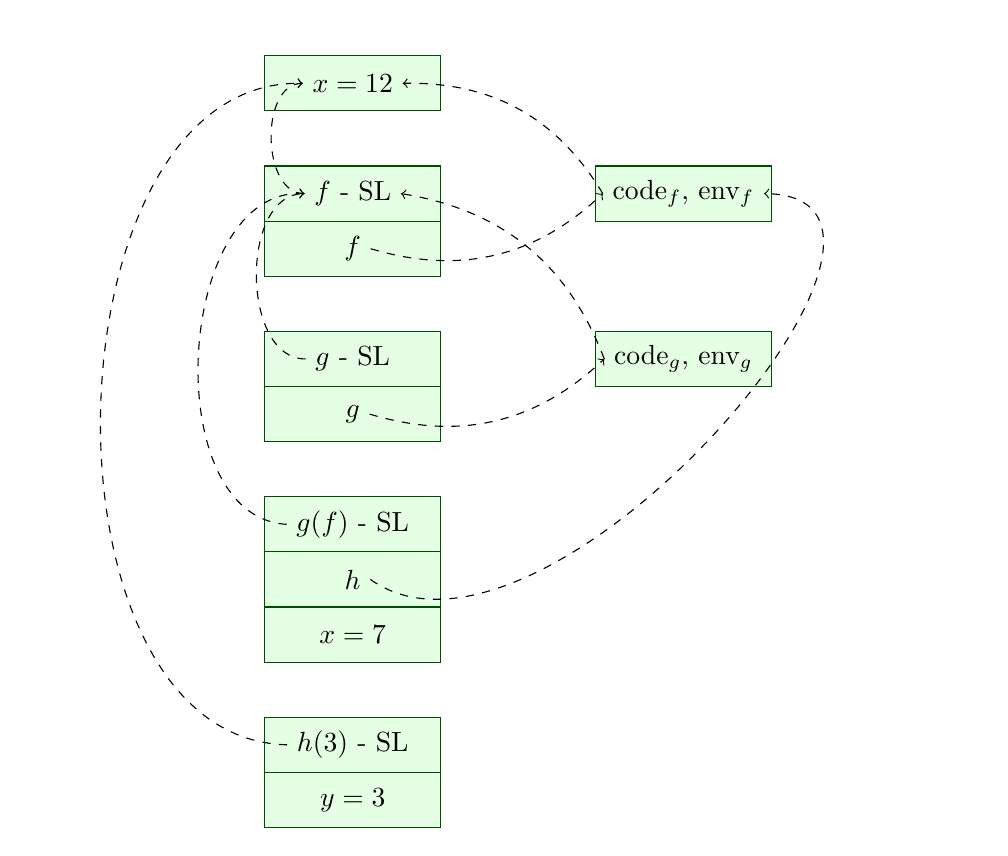
\begin{tikzpicture}[scale=.7]
    \drawstruct{(0, 0)}
    \structcell[freecell]{$x = 12$} 
    \coordinate (main) at (currentcell.west);
    \coordinate (main-e) at (currentcell.east);

    \drawstruct{(0, -2)}
    \structcell[freecell]{$f$ - SL} \coordinate (fw) at (currentcell.west); \coordinate (fse) at (currentcell.east);
    \structcell[freecell]{$f$} \coordinate (fe) at (currentcell.east);

    \drawstruct{(0, -5)}
    \structcell[freecell]{$g$ - SL} \coordinate (gw) at (currentcell.west); \coordinate (gse) at (currentcell.east);
    \structcell[freecell]{$g$} \coordinate (ge) at (currentcell.east);

    \drawstruct{(0, -8)}
    \structcell[freecell]{$g(f)$ - SL} \coordinate (gf) at (currentcell.west);
    \structcell[freecell]{$h$} \coordinate (h) at (currentcell.east);
    \structcell[freecell]{$x = 7$}

    \drawstruct{(0, -12)}
    \structcell[freecell]{$h(3)$ - SL} \coordinate (h3) at (currentcell.west);
    \structcell[freecell]{$y = 3$}

    \drawstruct{(6, -2)}
    \structcell[freecell]{code$_f$, env$_f$} 
    \coordinate (clos_f-w) at (currentcell.west);
    \coordinate (clos_f-e) at (currentcell.east);

    \drawstruct{(6, -5)}
    \structcell[freecell]{code$_g$, env$_g$} 
    \coordinate (clos_g-w) at (currentcell.west);
    \coordinate (clos_g-e) at (currentcell.east);

    \draw[->, dashed, bend right] (fw) to [out=90,in=90] (main);
    \draw[->, dashed, bend right] (gw) to [out=90,in=90] (fw);
    \draw[->, dashed, bend right] (gf) to [out=90,in=90] (fw);
    \draw[->, dashed, bend right] (h3) to [out=90,in=90] (main);

    \draw[->, dashed, bend right] (fe) to [out=-30,in=-150] (clos_f-w);
    \draw[->, dashed, bend right] (ge) to [out=-30,in=-150] (clos_g-w);
    \draw[->, dashed, bend left] (clos_f-w) to [out=-30,in=-150] (main-e);
    \draw[->, dashed, bend left] (clos_g-w) to [out=-30,in=-150] (fse);
    \draw[->, dashed, bend right] (h) to [out=-80,in=-45] (clos_f-e);

    % \draw[->, dashed, bend right] (A2)to [out=120,in=20] (main);
\end{tikzpicture}

\end{document}